% !TEX root = main.tex
\section{Experiments}

\subsection{Datasets and preprocessing}\label{app:experiments_setup}
% \todoe{This section also explain how we preprocessed the real-wolrd datasets too.}

We present here the datasets used in the article and how we preprocess them for numerical experiments conducted in Section \ref{sec:experiments}.

We consider two types of experiments, one on synthetic data with a contextual MAB problems with $K = 10$ arms such that for every arm $a$, $\theta_{a}$ is drawn from a folded normal distribution in dimension $d = 30$. We also use a finite number of contexts ($10$), each of them is drawn from a folded normal distribution projected on the unit circle multiplied by a uniform radius variable (i.i.d. across all contexts). Finally, we scale the expected rewards in $(0,1]$ and the noise is drawn from a centered Gaussian distribution $\mathcal{N}(0, 0.01)$. 
% The target arm is chosen at random among all arms. %I removed it because this is not always true 

The second type of experiments is conducted in the real-world datasets Jester \cite{goldberg2001eigentaste} and MovieLens25M \cite{harper2015movielens}. Jester consists of joke ratings on a continuous scale from $-10$ to $10$ for $100$ jokes from a total of $73421$ users. We use the features extracted via a low-rank matrix factorization ($d = 35$) to represent the actions (i.e., the jokes). We consider a complete subset of $40$ jokes and $19181$ users . Each user  rates all the $40$ jokes. At each time, a user is randomly selected from the $19181$ users and mean rewards are normalized in $[0, 1]$. The reward noise is $\mathcal{N} (0, 0.01)$. The second dataset we use is MovieLens25M. It contains $25000095$ ratings created by $162541$ users on $62423$ movies. We perform a low-rank matrix factorization to compute users features and movies features. We keep only movies with at least $1000$ ratings, which leave us with $162539$ users and $3794$ movies. At each time step, we present a random user, and the reward is the scalar product between the user feature and the recommend movie feature. All rewards are scaled to lie in $[0,1]$ and a Gaussian noise $\mathcal{N}(0, 0.01)$ is added to the rewards. 


\subsection{Attacks on Rewards}\label{app:additional_fig_rwds}
In this appendix, we present empirical evolution of the total cost and the number of draws for a unique target arm as a function of the attack parameter $\gamma$ for the Contextual ACE attack with perturbed rewards $\tilde{r}^{2}$ on generated data.

\begin{figure}[htbp]
    \centering
    \subfigure[Total cost]{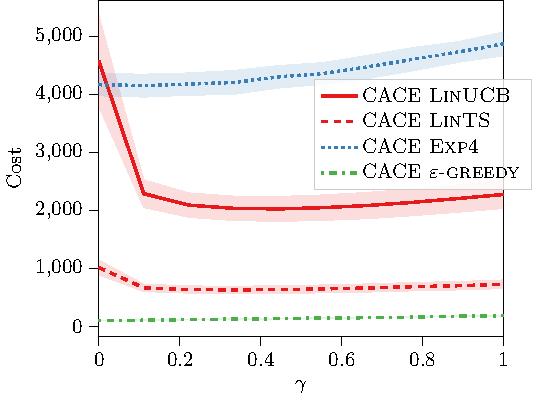
\includegraphics[width=0.35\textwidth]{sections/appendix/nips2020-bandits/images/attack_reward/simulations/cost_epsilon.pdf}}
    \subfigure[Number of draws]{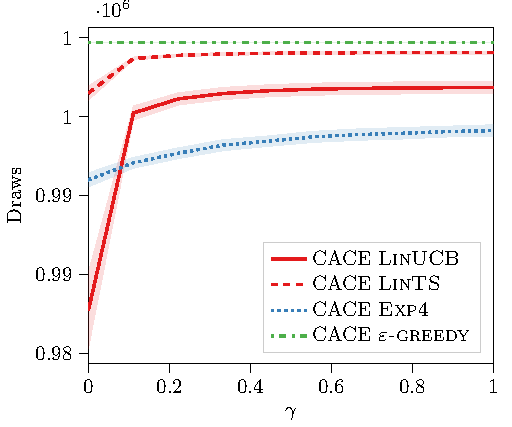
\includegraphics[width=0.3\textwidth]{sections/appendix/nips2020-bandits/images/attack_reward/simulations/draws_epsilon.pdf}}
    \caption{Total cost of attacks and number of draws of the target arm at $T = 10^{6}$ as a function of $\gamma$ on synthetic data     \label{fig:synth_cost_draws_gamma}
}
\end{figure}

Fig.~\ref{fig:synth_cost_draws_gamma} (left) shows that the total cost of attacks seems to be quite invariant w.r.t.  $\gamma$ except when $\gamma \rightarrow 0$ because the difference between the target arm and the other becomes negligible. This is also depicted by the total number of draws (Fig.~\ref{fig:synth_cost_draws_gamma}, Right) as the number of draws plummets when $\gamma \rightarrow 0$.

\begin{table}
\begin{center}
	\caption{\label{table:number_of_draws}Number of draws of the target arm $a^{\dagger}$ at $T=10^{6}$, for the synthetic data, $\gamma = 0.22$ for the Contextual ACE algorithm and for the Jester and MovieLens datasets $\gamma = 0.5$\otc{.}}
\begin{tabular}{lccc}
\toprule
{} & Synthetic &  Jester & Movilens \\
\midrule
\linucb          &      $86, 731.6$ &  $23, 548.16$ &    $25, 017.31$ \\
CACE \linucb     &     $996, 238.6$ &  $921, 083.69$ &   $944, 721.28$ \\
Stationary CACE \linucb &     $995, 578.88$ & $862, 095.67$ &   $931, 531.6$ \\
\epsgreedy       &     $111, 380.44$ & $21, 911.54$ &    $3, 165.81$    \\
CACE \epsgreedy  &    $999, 812.92$ &  $999, 755.72$ &   $999, 776.82$ \\
Stationary CACE \epsgreedy &     $999, 806.32$ &  $999, 615.98$ &   $999, 316.76$ \\
\lints           &      $91, 664.8$ &  $23, 398.3$ &    $30, 189.84$ \\
CACE \lints      &      $998, 997.04$ &   $976, 708.9$ &   $990, 250.67$ \\
Stationary CACE \lints &     $977, 850.96$ & $784, 715.62$ &   $845, 512.98$ \\
\expfour         &     $93, 860.4$ &  $29, 147.01$ &    $17, 985.78$ \\
CACE \expfour    &    $992, 793.36$ &   $989, 214.36$ &    $936, 230.4$ \\
Stationary CACE \expfour &     $993, 673.24$ &  $988, 463.56$ &   $934, 304.23$ \\
\bottomrule
\end{tabular}

\end{center}
\end{table}

\subsection{Attacks on all Contexts}\label{app:additional_fig_all_ctx}

% \begin{figure}[h]
%     \centering
%     \subfigure[Synthetic data]{\includegraphics[width=0.33\textwidth]{images/all_context_3_alg_sim/gen_cost_all.pdf}}\hfill
%     \subfigure[Jester Dataset]{\includegraphics[width=0.23\textwidth]{images/all_contexts_3_algs_jester/gen_jester_cost_all.pdf}}\hfill
%     \subfigure[MovieLens Dataset]{\includegraphics[width=0.23\textwidth]{images/all_contexts_3_alg_movielens/gen_movielens_cost_all.pdf}}
%     \caption{Total cost of the attacks for the attack of Sec.~\ref{sec:attack_all_context} on our synthetic dataset, Jester and MovieLens}
%     \label{fig:cost_all_algs_attack_all_ctx}
% \end{figure}

% Fig.~\ref{fig:cost_all_algs_attack_all_ctx} shows the total cost for all the attacks (that is to say including CC \lints and CC$20$ \lints compared to Fig~\ref{fig:costs_plot} (Right)). This figure shows that even though the total cost of attacks is linear for the synthetic and Jester dataset, it seems that for MovieLens the attacker achieves their goal with a logarithmic total. Therefore, despite the fact that the estimate of $\theta_{a^\dagger}$ can be polluted by attacked samples, it seems that \lints can still pick up $a^{\dagger}$ as being optimal for this particular instance.

\begin{figure}[ht]
   \begin{minipage}{0.25\linewidth}
        \centering
        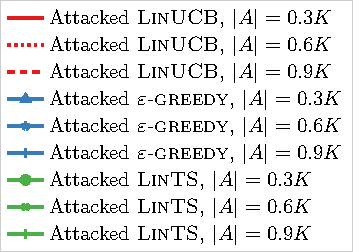
\includegraphics[width=0.85\linewidth]{sections/appendix/nips2020-bandits/images/regret_cost_attacks_context/simulations/legend.pdf}
        %\caption{Lorem ipsum}
    \end{minipage}\hfill
    \begin{minipage}{0.25\linewidth}
    \centering
    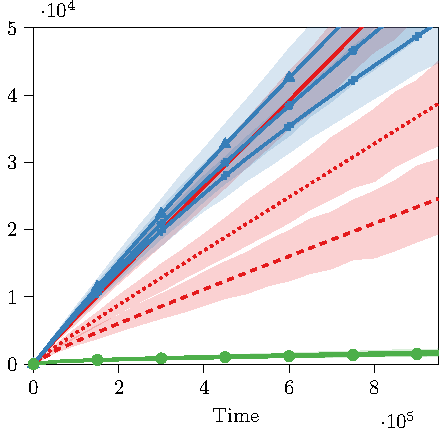
\includegraphics[width=0.95\linewidth]{sections/appendix/nips2020-bandits/images/regret_cost_attacks_context/simulations/standalone.pdf}
    % \caption{Synthetic}
    \end{minipage}\hfill
    \begin{minipage}{0.25\linewidth}
    \centering
    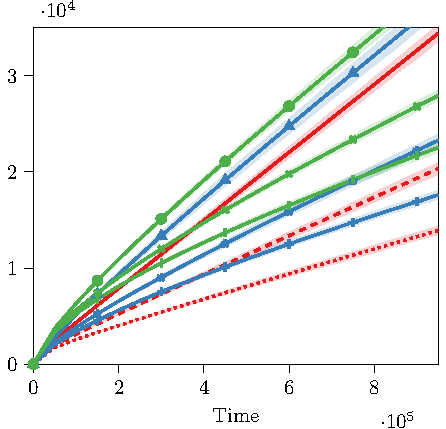
\includegraphics[width=0.85\linewidth]{sections/appendix/nips2020-bandits/images/regret_cost_attacks_context/jester/standalone.pdf}
    % \caption{Jester}
    \end{minipage}\hfill
    \begin{minipage}{0.25\linewidth}
    \centering
    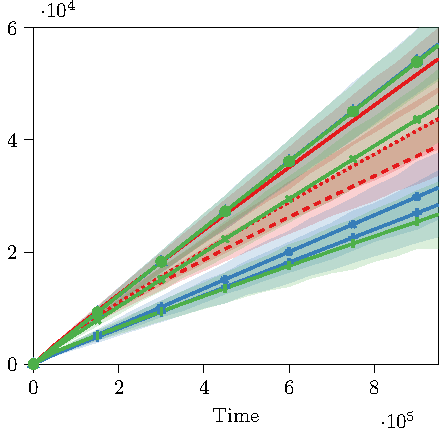
\includegraphics[width=0.85\linewidth]{sections/appendix/nips2020-bandits/images/regret_cost_attacks_context/movielens/standalone.pdf}
    % \caption{MovieLens}
    \end{minipage}
    \label{fig:regret_all_algs_attack_all_ctx}
\end{figure}

Fig.~\ref{fig:regret_all_algs_attack_all_ctx} shows the regret for all the attacks. This figure shows that even though the total cost of attacks is linear for algorithms like \lints in the synthetic dataset, the regret is linear. More generally, we observe that the regret is linear for all attacked algorithms on all datasets.

\subsection{Attack on a single context}\label{app:additional_fig_one_ctx}

The attacks are computed by solving the optimization problems \ref{eq:attack_one_user} and \ref{eq:relaxed_attack_one_user} (Sec.~\ref{sec:attack_one_context}). We choose the libraries according to their efficiency for each problem we need to solve. For Problem \eqref{eq:relaxed_attack_one_user} and Problem \eqref{eq:relaxed_TS_attack_one_user} we use \textsc{cvxpy}  \cite{cvxpy_rewriting} and the \textsc{ECOS} solver. %to solve the convex relaxations of the optimization problems for \linucb and \lints (equations \ref{eq:relaxed_attack_one_user}, \ref{eq:relaxed_TS_attack_one_user})
For Problem \eqref{eq:attack_one_user} we use the \textsc{SLSQP} method from the Scipy optimize library \cite{scipy} to solve the full \linucb problem (Equation \ref{eq:attack_one_user}) and \textsc{quadprog} to solve the quadratic problem to attack \epsgreedy.


\begin{figure}[htbp]
    \centering
    \subfigure[Synthetic data]{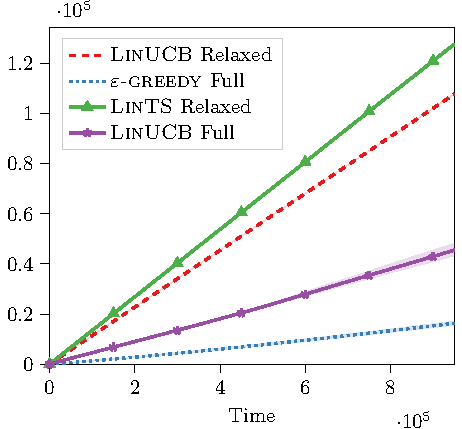
\includegraphics[width=0.33\textwidth]{sections/appendix/nips2020-bandits/images/one_context/simulations/standalone.pdf}}\hfill
    \subfigure[Jester Dataset]{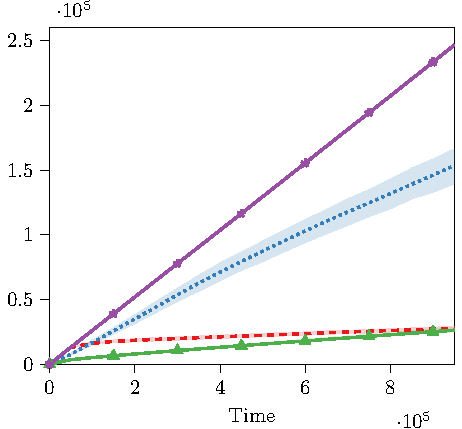
\includegraphics[width=0.33\textwidth]{sections/appendix/nips2020-bandits/images/one_context/jester/standalone.pdf}}\hfill
    \subfigure[MovieLens Dataset]{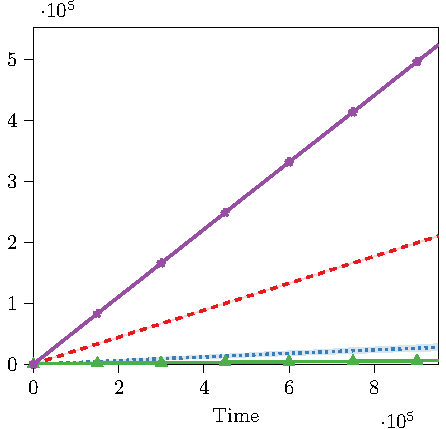
\includegraphics[width=0.33\textwidth]{sections/appendix/nips2020-bandits/images/one_context/movielens/standalone.pdf}}
    \caption{Total cost of the attacks for the attacks one one context on our synthetic dataset, Jester and MovieLens. As expected, the total cost is linear.     \label{fig:cost_attack_one_ctx}}
\end{figure}